% basic style definitions for lecture notes in presentation mode.
% based on material from J. W. Langelaan, August 16, 2010

% Vitor Valente, August 2024

\documentclass[times,12pt]{beamer}

\setbeamercolor{background canvas}{bg=white} % Background is set to white
\setbeamercolor{normal text}{fg=black}
\setbeamercolor{alerted text}{fg=black}
\setbeamercolor{example text}{fg=black}
\setbeamercolor{structure}{fg=black} % Section headers, etc.

\setbeamerfont{section title}{size=\small}
\setbeamerfont{frametitle}{size=\large}
\setbeamerfont{normal text}{size=\small}

\setbeamertemplate{navigation symbols}{}

\setbeamertemplate{itemize subitem}[circle]

\setbeamerfont{normal text}{size=\footnotesize}
\setbeamerfont{itemize item}{size=\footnotesize}
\setbeamerfont{itemize text}{size=\footnotesize}

\usepackage{graphicx}
\usepackage{amsmath}  % For mathematical symbols
\usepackage{graphicx} % For including images
\usepackage{hyperref} % For clickable links
\usepackage{subcaption}
\usepackage{tikz} % For block diagrams
\usetikzlibrary{positioning}

\usepackage{ragged2e}
\apptocmd{\frame}{}{\justifying}{} % Allow optional arguments after frame.

\usepackage{xcolor}

% define an environment that prints out notes to self in red if \printnotes is true, in white (on white paper,
% hence invisible) otherwise. Printing notes in white will leave space for student notes...
\newif\ifprintnotes
\newenvironment{mynotes}
{
	\ifprintnotes
		\color{red}
	\else
		\color{white}
	\fi
}
{
	\color{black}
}

% !TEX root = Lecture02.tex
\usepackage{pgfpages}
\usepackage[absolute,overlay]{textpos}

\usetikzlibrary{calc}
\usetikzlibrary{arrows.meta, positioning}

% For printing purposes, 2 slides per page with borders
\pgfpagesuselayout{2 on 1}[letterpaper,border shrink=5mm]
\pgfpageslogicalpageoptions{1}{border code=\pgfusepath{stroke}}
\pgfpageslogicalpageoptions{2}{border code=\pgfusepath{stroke}}
\pgfpageslogicalpageoptions{3}{border code=\pgfusepath{stroke}}
\pgfpageslogicalpageoptions{4}{border code=\pgfusepath{stroke}}

% Title Page Information
\title[AERSP304]{Reference Frames and Time Derivatives of a Vector}
\subtitle{AERSP 304 - Dynamics and Control of \\ Aerospace Systems}
\author[V. T. Valente]{V.T. Valente}
\institute[Penn State University]{Penn State University}
\date{January 14, 2026}

\setlength{\itemsep}{0.0cm}
\setlength{\parsep}{0cm}

\begin{document}
{
%\setbeamertemplate{footline}[text line]{\parbox{\linewidth}{\vspace*{-8pt}Some material in this presentation has been adapted from slides developed by Dr. Joe Horn.}}
\frame{\titlepage}
}

\small

% \begin{center}
%     \begin{tikzpicture}[scale=0.95, line cap=round, line join=round]
%         % origin
%         \coordinate (O) at (0,0);

%         % inertial (N) axes
%         \draw[->, thick] (O) -- (-1.4,-1.2) node[left]  {$\hat{\mathbf n}_1$};
%         \draw[->, thick] (O) -- ( 2.0, 0.0) node[right] {$\hat{\mathbf n}_2$};
%         \draw[->, thick] (O) -- ( 0.0, 2.0) node[above left] {$\hat{\mathbf n}_3$};

%         % body (B) axes
%         \draw[->, thick, blue] (O) -- ( -0.4,-1.4) node[below right] {$\hat{\mathbf b}_1$};
%         \draw[->, thick, blue] (O) -- ( 1.8, 0.8) node[above right] {$\hat{\mathbf b}_2$};
%         \draw[->>, thick, blue] (O) -- ( 0.0, 2.0) node[above right] {$\hat{\mathbf b}_3$};

%         % angle between b2 and n2
%         \draw[->] (0.9,0.0) arc[start angle=0, end angle=23, radius=0.9];
%         \node at (1.1,0.25) {\scriptsize$\theta$};
%     \end{tikzpicture}
% \end{center}

\begin{frame}{Goals for Today}
    \begin{itemize}
        \item Review the definition of Frame of References
        \item Review the definition of DCMs
        \item Understand time derivatives of vectors in different frames of reference
    \end{itemize}
\end{frame}

\begin{frame}[t]{Reference Frames}
\small
A \emph{frame} is a language used to convey dynamical information.
\vspace{0.5cm}

\begin{tikzpicture}[scale=0.95, line cap=round, line join=round]
    % origin
    \coordinate (O) at (0,0);

    % inertial (N) axes
    \draw[->, thick] (O) -- (-1.4,-1.2) node[left]  {$\hat{\mathbf n}_1$};
    \draw[->, thick] (O) -- ( 2.0, 0.0) node[right] {$\hat{\mathbf n}_2$};
    \draw[->, thick] (O) -- ( 0.0, 2.0) node[above left] {$\hat{\mathbf n}_3$};

    % % body (B) axes
    % \draw[->, thick, blue] (O) -- ( -0.4,-1.4) node[below right] {$\hat{\mathbf b}_1$};
    % \draw[->, thick, blue] (O) -- ( 1.8, 0.8) node[above right] {$\hat{\mathbf b}_2$};
    % \draw[->>, thick, blue] (O) -- ( 0.0, 2.0) node[above right] {$\hat{\mathbf b}_3$};

    % % angle between b2 and n2
    % \draw[->] (0.9,0.0) arc[start angle=0, end angle=23, radius=0.9];
    % \node at (1.1,0.25) {\scriptsize$\theta$};
\end{tikzpicture}

\end{frame}

\begin{frame}[t]{Reference Frames Continued}
    How is $B$ oriented w.r.t.\ $N$?
\end{frame}

\begin{frame}[t]{Direction Cosine Matrix (DCM)}

\end{frame}

\begin{frame}[t]{What is the orientation of $N$ w.r.t. $B$?}

\end{frame}

\begin{frame}[t]{What about another frame ($A$) rotating w.r.t. $B$?}

\end{frame}

\begin{frame}[t]{Reference Frames and Independent Parameters}

\end{frame}

\begin{frame}[t]{Time Derivative of a Vector}
    \begin{flushright}
    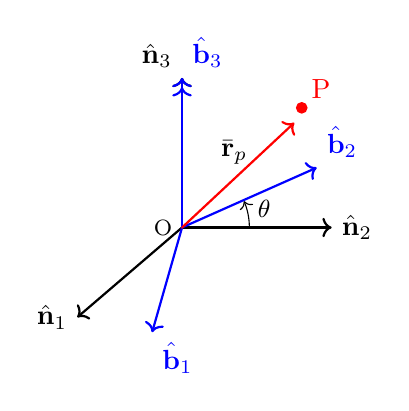
\begin{tikzpicture}[scale=0.95, line cap=round, line join=round]
        % origin
        \coordinate (O) at (0,0);
        \node at (O) [left] {\footnotesize$\text{O}$};

        % inertial (N) axes
        \draw[->, thick] (O) -- (-1.4,-1.2) node[left]  {$\hat{\mathbf n}_1$};
        \draw[->, thick] (O) -- ( 2.0, 0.0) node[right] {$\hat{\mathbf n}_2$};
        \draw[->, thick] (O) -- ( 0.0, 2.0) node[above left] {$\hat{\mathbf n}_3$};

        % body (B) axes
        \draw[->, thick, blue] (O) -- ( -0.4,-1.4) node[below right] {$\hat{\mathbf b}_1$};
        \draw[->, thick, blue] (O) -- ( 1.8, 0.8) node[above right] {$\hat{\mathbf b}_2$};
        \draw[->>, thick, blue] (O) -- ( 0.0, 2.0) node[above right] {$\hat{\mathbf b}_3$};

        % angle between b2 and n2
        \draw[->] (0.9,0.0) arc[start angle=0, end angle=23, radius=0.9];
        \node at (1.1,0.25) {\small$\theta$};

        % add vector r_p
        \draw[->, thick, red] (O) -- (1.5,1.4);
        \node at (1.0,1.0) [left] {$\bar{\mathbf r}_p$};
        % add point P at the end
        \filldraw[red] (1.6,1.6) circle (2pt) node[above right] {P};
    \end{tikzpicture}
    \end{flushright}
\end{frame}

\begin{frame}[t]{Transport Theorem}

\end{frame}

\begin{frame}{Summary}
    \textbf{Basis vectors:} orthonormal, dextral (right-handed)
    \[
        \hat{\mathbf n}_1 \times \hat{\mathbf n}_2 = \hat{\mathbf n}_3
    \]

    \textbf{DCM:} maps coordinates \emph{to $B$ from $N$}

    \[
    \begin{bmatrix}
        {\mathbf x}_B\\[0.2em]
        {\mathbf y}_B\\[0.2em]
        {\mathbf z}_B
    \end{bmatrix}
      =
    \underbrace{\begin{bmatrix}
        \hat{\mathbf b}_1\!\cdot\!\hat{\mathbf n}_1 & \hat{\mathbf b}_1\!\cdot\!\hat{\mathbf n}_2 & \hat{\mathbf b}_1\!\cdot\!\hat{\mathbf n}_3\\
        \hat{\mathbf b}_2\!\cdot\!\hat{\mathbf n}_1 & \hat{\mathbf b}_2\!\cdot\!\hat{\mathbf n}_2 & \hat{\mathbf b}_2\!\cdot\!\hat{\mathbf n}_3\\
        \hat{\mathbf b}_3\!\cdot\!\hat{\mathbf n}_1 & \hat{\mathbf b}_3\!\cdot\!\hat{\mathbf n}_2 & \hat{\mathbf b}_3\!\cdot\!\hat{\mathbf n}_3
    \end{bmatrix}}_{C_{BN}}
    \begin{bmatrix}
        {\mathbf x}_N\\[0.2em]
        {\mathbf y}_N\\[0.2em]
        {\mathbf z}_N
    \end{bmatrix}
    \]
    \[
        \hat{\mathbf b} = C_{BN}\,\hat{\mathbf n}, \quad \hat{\mathbf n} = C_{NB}\,\hat{\mathbf b}
    \]
    \[
        C_{NB} = \left(C_{BN}\right)^{-1},
        \qquad
        C_{NB} = \left(C_{BN}\right)^{T}.
    \]
    \[
        \hat{\mathbf a} = \underbrace{C_{AB}\,C_{BN}}_{C_{AN}}\,\hat{\mathbf n}.
    \]
\end{frame}



% Frame 4 ------------------------------------------------------------
\begin{frame}{Summary Continued}
\small
Let
\[
  \mathbf r_p = x\,\hat{\mathbf b}_1 + y\,\hat{\mathbf b}_2 + z\,\hat{\mathbf b}_3.
\]

Differentiate:
\[
  \frac{d\mathbf r_p}{dt}
  = \dot{x}\,\hat{\mathbf b}_1 + x\,\dot{\hat{\mathbf b}}_1
  + \dot{y}\,\hat{\mathbf b}_2 + y\,\dot{\hat{\mathbf b}}_2
  + \dot{z}\,\hat{\mathbf b}_3 + z\,\dot{\hat{\mathbf b}}_3.
\]


Transport theorem (applied to \(\hat{\mathbf b}_i\)):
\[
  {}^{N}\frac{d\hat{\mathbf b}}{dt}
  =
  {}^{B}\frac{d\hat{\mathbf b}}{dt}
  +
  \boldsymbol\omega_{B/N}\times \hat{\mathbf b}.
\]

Hence,
\[
  \boxed{
  {}^{N}\dot{\mathbf r}_p
  =
  {}^{B}\dot{\mathbf r}_p
  +
  \boldsymbol\omega_{B/N}\times \mathbf r_p
  }
\]
\end{frame}

\end{document}
